% This file was created with tikzplotlib v0.10.1.
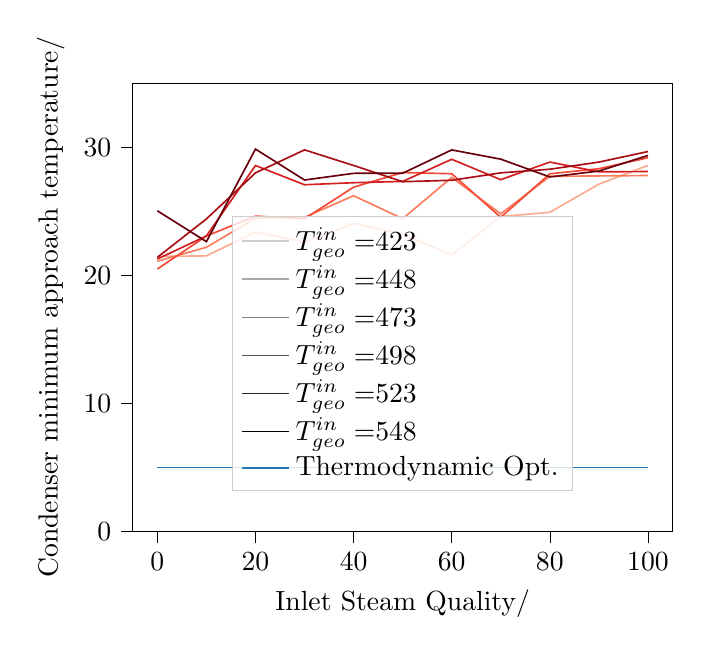
\begin{tikzpicture}

\definecolor{coral25112593}{RGB}{251,125,93}
\definecolor{crimson2113132}{RGB}{211,31,32}
\definecolor{darkgray168}{RGB}{168,168,168}
\definecolor{darkgray176}{RGB}{176,176,176}
\definecolor{darkslategray41}{RGB}{41,41,41}
\definecolor{dimgray89}{RGB}{89,89,89}
\definecolor{firebrick1681521}{RGB}{168,15,21}
\definecolor{gray127}{RGB}{127,127,127}
\definecolor{lightgray204}{RGB}{204,204,204}
\definecolor{lightgray206}{RGB}{206,206,206}
\definecolor{lightsalmon252171142}{RGB}{252,171,142}
\definecolor{maroon103012}{RGB}{103,0,12}
\definecolor{steelblue31119180}{RGB}{31,119,180}
\definecolor{tomato2437554}{RGB}{243,75,54}

\begin{axis}[
legend cell align={left},
legend style={
  fill opacity=0.8,
  draw opacity=1,
  text opacity=1,
  at={(0.5,0.09)},
  anchor=south,
  draw=lightgray204
},
tick align=outside,
tick pos=left,
x grid style={darkgray176},
xlabel={Inlet Steam Quality/\unit{\percent}},
xmin=-5, xmax=105,
xtick style={color=black},
y grid style={darkgray176},
ylabel={Condenser minimum approach temperature/\unit{\K}},
ymin=0, ymax=35,
ytick style={color=black}
]
\addplot [semithick, lightgray206]
table {%
0 -1
1 -1
};
\addlegendentry{\(T_{geo}^{in}=\)\qty{423}{\K}}
\addplot [semithick, lightsalmon252171142, forget plot]
table {%
0 21.477693690657
10 21.516203103838
20 23.3776950121904
30 22.5939381327143
40 24.0531021944763
50 23.2025880174416
60 21.59941031362
70 24.5927744914032
80 24.9192024808735
90 27.1153552191322
100 28.5757311977719
};
\addplot [semithick, darkgray168]
table {%
0 -1
1 -1
};
\addlegendentry{\(T_{geo}^{in}=\)\qty{448}{\K}}
\addplot [semithick, coral25112593, forget plot]
table {%
0 21.1005872595034
10 22.1895163211857
20 24.4560746478686
30 24.5306942098682
40 26.2140837942385
50 24.4177148350573
60 27.6432915426399
70 24.8010573346589
80 27.7277120690675
90 27.7585803630629
100 27.7910844860225
};
\addplot [semithick, gray127]
table {%
0 -1
1 -1
};
\addlegendentry{\(T_{geo}^{in}=\)\qty{473}{\K}}
\addplot [semithick, tomato2437554, forget plot]
table {%
0 20.4899769126707
10 23.0688525352336
20 24.6197294934274
30 24.4177148350573
40 26.8809487432662
50 28.022670322494
60 27.931082697435
70 24.5241543075799
80 27.9275238192777
90 28.3209271291002
100 29.178323032567
};
\addplot [semithick, dimgray89]
table {%
0 -1
1 -1
};
\addlegendentry{\(T_{geo}^{in}=\)\qty{498}{\K}}
\addplot [semithick, crimson2113132, forget plot]
table {%
0 21.2688722310976
10 23.0719844000401
20 28.5713775512313
30 27.0703274918728
40 27.2298353506859
50 27.330702041515
60 29.056712917268
70 27.4676495547989
80 28.8407866227749
90 28.0792904190134
100 28.1017830769427
};
\addplot [semithick, darkslategray41]
table {%
0 -1
1 -1
};
\addlegendentry{\(T_{geo}^{in}=\)\qty{523}{\K}}
\addplot [semithick, firebrick1681521, forget plot]
table {%
0 21.4022921735182
10 24.4031776279197
20 27.9957652291495
30 29.7937737909401
40 28.5740034472093
50 27.307388008633
60 27.4188975700408
70 27.9991573926123
80 28.2806255438038
90 28.838797816093
100 29.6612520171413
};
\addplot [semithick, black]
table {%
0 -1
1 -1
};
\addlegendentry{\(T_{geo}^{in}=\)\qty{548}{\K}}
\addplot [semithick, maroon103012, forget plot]
table {%
0 25.035044694954
10 22.6286164997631
20 29.8554530172785
30 27.4389842257544
40 27.9613786274637
50 27.9681627613132
60 29.7893217104112
70 29.0673588298923
80 27.6780752995856
90 28.14074625524
100 29.3563569232359
};
\addplot [semithick, steelblue31119180]
table {%
0 5
100 5
};
\addlegendentry{Thermodynamic Opt.}
\end{axis}

\end{tikzpicture}
